% §5.4 Invariant wedges --- blueprint chapter 5, part 05-wedges.tex (Q-0288). Included from
% 05-landscape.tex; the conventions are in that file's header. The nodes are linear algebra; since
% Q-0281 wave 2, group F (the author's decision of 2026-10-05) lem:spectral-cones(2) cites C4 (ledger
% A9) in place of its compound-matrix proof, and the nodes that read it spend it. Q-0290: lem:spectral-cones, thm:cone-orders (whole, the node not
% being split; this file states its four clauses in words) and the proof of prop:invariant-orders are
% in appendix A; prop:stable-order-generated is in 5.6, after the exponent cone it reads (review flag
% S12). The prior-art paragraph cites the readings recorded in
% records/affine/READING-{lawson1989ordered,hilgert1989lie,hilgert1997causal,faraut1994analysis}.md,
% with the page anchors of the nodes' annotations; no proof depends on them. The chain of cones and
% the general linear row along it (thm:wedge-axis) are stated in 5.3.
% Q-0309 (fix group 2, review flag 35): thm:cone-orders is stated here, in place of the paraphrase of
% its four clauses, since its clause (4) defines the order thm:wedge-axis is stated on; its proof,
% lem:spectral-cones and the proof of prop:invariant-orders are in the proof appendix (app:proofs).

\subsection{Invariant wedges}\label{sec:invariant-wedges}

An order of the landscape says which changes of aperture must be further smoothings. This subsection
asks which orders there are, and how to describe one by what may happen in an instant. For the
Gaussian the answer is familiar. Its aperture may grow in any direction, $\Sigma(t)$ moving with a
positive semidefinite velocity $\Sigma'(t)$, and the pairs joined by such a curve are those of the
Loewner order (Proposition~\ref{prop:stable-order-generated}(1), at $\alpha = \infty$). The rays allow
only a velocity that is a nonnegative multiple of $\Sigma(t)$, a growth without a change of shape. An
order in between allows at each aperture a cone of velocities, the \emph{cone field}, and relates two
apertures when a curve whose velocity stays in the cones joins them. The main result,
Theorem~\ref{thm:cone-orders}, says that the closed invariant partial orders on $\PD(d)$ that arise
in this way are exactly those whose steps can be taken in fractions, and that every step of such an
order is reached along one curve, with no limit of curves needed. The rays, the stable orders and the
Loewner order are of this kind, the members $C_0$, $C_\alpha$ and $C_\infty$ of one chain of cones
(Proposition~\ref{prop:stable-order-generated}).

% Pass 6, the author's review of section 4.4 (2026-11-02; records/affine/REVIEW-author-paper-affine.md):
% "some, preferably geometric, intuition about what the cone and wedges are and how they will be
% used". Paper-only prose. The plane computation: X = [[a+u, v], [v, a-u]] has eigenvalues
% a +- r, r = sqrt(u^2+v^2); a rotation by phi rotates (u, v) by 2 phi and fixes a, a reflection
% reflects (u, v); so an O(2)-invariant closed convex cone with I in it and no line is
% {r <= k a}, k >= 0. PSD(2) is k = 1. C_alpha of prop:stable-order-generated, (2+alpha) lambda_min
% >= tr, is (2+alpha)(a-r) >= 2a, that is k = alpha/(alpha+2): C_0 has k = 0, C_2 has k = 1/2, and
% k -> 1 as alpha -> infinity. thm:wedge-axis(2) read in the plane: beta(C) = max tr X/lambda_min(X)
% - 2 = 2k/(1-k) for the round cone of opening k < 1, so (a) k > 1 (not in PSD(2)): no family;
% (b) k = 1 (a singular member): the Gaussian only; (c) k < 1: a non-Gaussian family exists iff
% beta < 2 iff k < 1/2.
\paragraph{A picture in the plane.} For $d = 2$ the cones can be drawn. Write a symmetric matrix as
$X = \bigl(\begin{smallmatrix} a+u & v \\ v & a-u \end{smallmatrix}\bigr)$, so that $\Sym(2)$ is a
space of three dimensions with coordinates $(a, u, v)$, and $X$ has the eigenvalues
$a \pm \sqrt{u^2+v^2}$. Read $X$ as the velocity of an aperture at $I$. Then $a$ is its growth in
size, $\sqrt{u^2+v^2}$ its rate of change of shape, and the angle of $(u, v)$ the direction in which
it stretches. A rotation of the plane by an angle $\phi$ rotates $(u, v)$ by $2\phi$ and leaves $a$
alone. So a closed convex cone that is invariant under rotations, contains $I$ and contains no line is
a round cone about the axis of the multiples of $I$,
\[
  \sqrt{u^2+v^2} \le k\,a \qquad \text{for some } k \ge 0 .
\]
Its opening $k$ bounds how fast the shape may change against how fast the aperture grows
(Figure~\ref{fig:cones-plane}). The rays
are the axis alone, $k = 0$. The Loewner order allows every positive semidefinite velocity, the cone
$k = 1$ of half-angle $45^\circ$, and a wider cone allows an aperture to shrink in some direction. The
cone $C_\alpha$ of the chain has $k = \alpha/(\alpha+2)$, so the stable orders, $0 < \alpha < 2$, are
the cones narrower than $k = \frac12$. The cone field carries the cone at $I$ to every aperture by the
group, and the order relates two apertures when a curve whose velocity stays in the cones joins them.
Lie theory calls a closed convex cone a \emph{wedge} (\S\ref{sec:affine-covariance}), and these
wedges, which contain no line, are the tangent objects through which it studies such orders. The rest
of the section uses them in two ways. Each affine orbit has its own set of steps along which it
cascades, and \S\S\ref{sec:affine-orbits}--\ref{sec:affine-stable-cone} find it for the orbits of
interest: the rays alone for the \Matern{} kernels, the order of $C_\gamma$ for the stable kernel of
index $\gamma$. And in the plane
Theorem~\ref{thm:wedge-axis} reads off the opening. A cone with $k < \frac12$ carries non-Gaussian
families, a cone with $\frac12 \le k \le 1$ carries only the affine Gaussian scale spaces, and a cone
with $k > 1$ carries none.

% Pass 6 (the author's request of 2026-11-02, "Add the figure please"): fig-cones-plane.png, drawn by
% records/affine/fig-cones-plane.py with its output saved (fig-cones-plane-output.txt); the script
% checks the openings k = alpha/(alpha+2), PSD(2) = {r <= a} and beta = 2k/(1-k) before drawing. No
% statement uses it.
\begin{figure}[t]
\centering
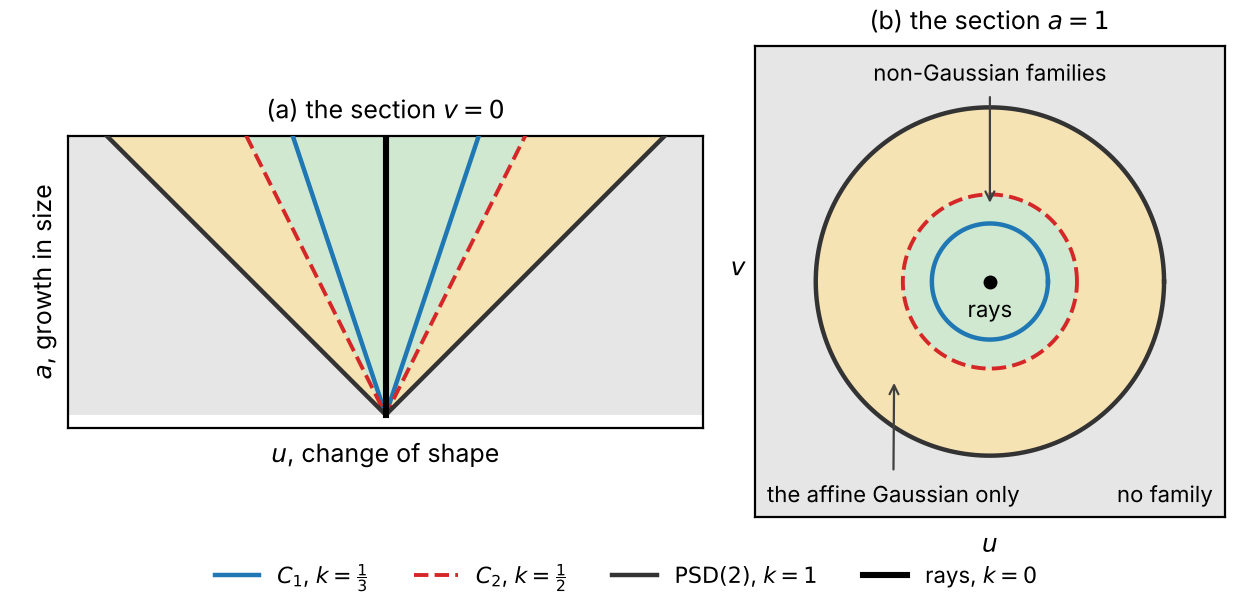
\includegraphics[width=\textwidth]{fig-cones-plane.png}
\caption{The rotation-invariant cones of velocities in the plane, in the coordinates $(a, u, v)$ of
$X = \bigl(\begin{smallmatrix} a+u & v \\ v & a-u \end{smallmatrix}\bigr)$: each is a round cone
$\sqrt{u^2+v^2} \le k\,a$ about the axis of the multiples of $I$. (a) The section $v = 0$, where each
cone is a sector. (b) The section $a = 1$, where each cone is a disc of radius $k$. Drawn are the rays
($k = 0$), the cone $C_1$ ($k = \frac13$), along whose order the orbit of the Poisson kernel cascades,
the cone $C_2$ ($k = \frac12$) and the Loewner cone $\PSD(2)$ ($k = 1$). The shading reads
Theorem~\ref{thm:wedge-axis} in the plane: a cone with $k < \frac12$ (green) carries non-Gaussian
families, one with $\frac12 \le k \le 1$ (amber) only the affine Gaussian scale spaces, and one with
$k > 1$ (grey) none. Drawn by a script deposited with the paper.}
\label{fig:cones-plane}
\end{figure}

The rest of the subsection is linear algebra, in the language of matrix analysis and of the Lie theory
of semigroups, where the orders of a homogeneous space are studied through their cones (``Prior art''
at the end of the subsection).
% Round 2 (presentation review), item 19 (VERIFY-round2-notation-paper.md § 19): the motivation of
% causal curves and of majorization, compared with Theorem 4.3(1) (the test log M in C is its
% conclusion, the order being defined by curves) and Lemma C.1(2), (5).
An order is described by its set of relative steps $M = \Sigma^{-1/2}\Sigma'\Sigma^{-1/2}$
(Proposition~\ref{prop:invariant-orders}), and an $\Orth(d)$-invariant closed convex cone $C$ of symmetric matrices plays
the part of the allowed velocities, through the cone field of Theorem~\ref{thm:cone-orders}. A single
step is tested by its logarithm: Theorem~\ref{thm:cone-orders}(1) shows that a curve of that cone
field joins $\Sigma$ to $\Sigma'$ exactly when $\log M \in C$. Steps do not compose by multiplication.
The composite of two steps $M$ and $N$ is $M^{1/2}N'M^{1/2}$ with $N'$ a rotation of $N$
(Proposition~\ref{prop:invariant-orders}(3)), and its logarithm is not $\log M + \log N'$ when $M$
and $N'$ do not commute. So it is not obvious that the test is transitive. A comparison of spectra by partial sums,
majorization, bounds the spectrum of the composite whatever the relative position of the eigenframes,
with one cited inequality (C4, Theorem~\ref{thm:cited-A9}). It gives both the transitivity and the
fact that a curve of the cone field ends at a step in $\exp C$.
Proposition~\ref{prop:invariant-orders} sets up the dictionary between invariant orders and sets of
steps in which the theorem is stated.

% shared with blueprint prop:invariant-orders
\begin{proposition}[invariant relations on $\PD(d)$ and their steps]\label{prop:invariant-orders}
Let $d \ge 1$ and write $\Sym(d)$ for the real symmetric $d \times d$ matrices. Call a set
$\mathcal K \subseteq \PD(d)$ a \emph{step set} if $QMQ^{\tp} \in \mathcal K$ whenever $M \in \mathcal K$
and $Q \in \Orth(d)$. For a step set write $\Sigma \le_{\mathcal K} \Sigma'$, for
$\Sigma, \Sigma' \in \PD(d)$, when the \emph{relative step} $\Sigma^{-1/2}\Sigma'\Sigma^{-1/2}$ lies in
$\mathcal K$, and put $\mathcal S_{\mathcal K} := \{A \in \GL(d) : AA^{\tp} \in \mathcal K\}$.
\begin{enumerate}
\item \emph{(Invariant relations are step sets.)} For $\Sigma, \Sigma' \in \PD(d)$ and every
$A \in \GL(d)$ with $AA^{\tp} = \Sigma$, $\Sigma \le_{\mathcal K} \Sigma'$ if and only if
$A^{-1}\Sigma'A^{-\tp} \in \mathcal K$. The relation $\le_{\mathcal K}$ is $\GL(d)$-invariant:
$\Sigma \le_{\mathcal K} \Sigma'$ if and only if $B\Sigma B^{\tp} \le_{\mathcal K} B\Sigma'B^{\tp}$, for
every $B \in \GL(d)$. Every $\GL(d)$-invariant relation $R$ on $\PD(d)$ is $\le_{\mathcal K}$ for
exactly one step set, $\mathcal K = \{M \in \PD(d) : I \,R\,M\}$.
\item \emph{(Order properties.)} $\le_{\mathcal K}$ is reflexive if and only if $I \in \mathcal K$; it is
antisymmetric if and only if no $M \ne I$ has both $M$ and $M^{-1}$ in $\mathcal K$; and it is closed in
$\PD(d) \times \PD(d)$ if and only if $\mathcal K$ is closed in $\PD(d)$.
\item \emph{(How steps compose.)} If $\Sigma \le_{\mathcal K} \Sigma' \le_{\mathcal K} \Sigma''$, $M$ is
the relative step of $(\Sigma, \Sigma')$ and $N$ that of $(\Sigma', \Sigma'')$, then the relative step
of $(\Sigma, \Sigma'')$ is $M^{1/2}N'M^{1/2}$ with $N' = Q^{\tp}NQ$ for some $Q \in \Orth(d)$, and its
eigenvalues are those of $MN'$. Conversely, for $M, N \in \mathcal K$ the triple $I$, $M$,
$M^{1/2}NM^{1/2}$ is such a chain. So $\le_{\mathcal K}$ is transitive if and only if
$M^{1/2}NM^{1/2} \in \mathcal K$ for all $M, N \in \mathcal K$, if and only if $\mathcal S_{\mathcal K}$
is closed under products. The spectrum of the composite is not determined by the spectra of the two
steps: for $d = 2$ the step $\diag(4,1)$ followed by $\diag(4,1)$ gives $\diag(16,1)$, and followed by
$\diag(1,4)$ gives $4I$.
\item \emph{(The infinitesimal cone.)} The set
$C(\mathcal K) := \{X \in \Sym(d) : e^{tX} \in \mathcal K \text{ for every } t \ge 0\}$ is invariant
under $X \mapsto QXQ^{\tp}$, $Q \in \Orth(d)$, and under $X \mapsto cX$, $c \ge 0$. It is closed when
$\mathcal K$ is closed in $\PD(d)$, and if $\le_{\mathcal K}$ is antisymmetric then
$X \in C(\mathcal K)$ and $-X \in C(\mathcal K)$ only for $X = 0$.
\end{enumerate}
\end{proposition}

Clause (1) is the dictionary between the orders of the scheme and sets of matrices: a
$\GL(d)$-invariant order on $\PD(d) = \GL(d)/\Orth(d)$ is its set of relative steps at $I$.
The proof is in Appendix~\ref{app:wedge-axis}.

The invariant cones are read through their eigenvalues. For $X \in \Sym(d)$ write
$\lambda^\uparrow(X)$ for its eigenvalues in increasing order, and for a cone $C \subseteq \Sym(d)$
put $\exp C := \{e^X : X \in C\}$.

An invariant cone generates an order along curves that move in the cone at each point. The theorem
says which orders arise in this way, and its clause (4) gives the orders on $\PSD(d)$ along which the
general linear row is read in \S\ref{sec:wedge-axis-proof}.

% CHANGED Q-0281 wave 2: blind review W2F-4 (the sentence above) and W2F-5 (the parenthetical of clause
% (3), mirrored from the blueprint statement).
% shared with blueprint thm:cone-orders
\begin{theorem}[invariant orders generated by cone fields]\label{thm:cone-orders}
Let $d \ge 1$ and let $C \subseteq \Sym(d)$ be a closed convex cone invariant under $X \mapsto QXQ^{\tp}$,
$Q \in \Orth(d)$. Its \emph{cone field} assigns to $\Sigma \in \PD(d)$ the cone
$\Sigma^{1/2}C\Sigma^{1/2}$ of tangent vectors, which equals $ACA^{\tp}$ for every $A$ with
$AA^{\tp} = \Sigma$, so that $B(\Sigma^{1/2}C\Sigma^{1/2})B^{\tp}$ is the cone at $B\Sigma B^{\tp}$ for
$B \in \GL(d)$. An absolutely continuous $\gamma : [0,1] \to \PD(d)$ is \emph{$C$-causal} if
$\gamma(t)^{-1/2}\gamma'(t)\gamma(t)^{-1/2} \in C$ for almost every $t$; write $\Sigma \preceq_C \Sigma'$
when a $C$-causal curve runs from $\Sigma$ to $\Sigma'$. Use the notation of Proposition~\ref{prop:invariant-orders}
(step sets $\mathcal K$, their relations $\le_{\mathcal K}$, the sets $\mathcal S_{\mathcal K}$ and the cones
$C(\mathcal K)$), write $\exp C := \{e^X : X \in C\}$, and write $\lambda^\uparrow_1(M)$ for the least
eigenvalue of $M$.
\begin{enumerate}
\item \emph{(The order of a cone field.)} $\Sigma \preceq_C \Sigma'$ if and only if the relative step
$M = \Sigma^{-1/2}\Sigma'\Sigma^{-1/2}$ lies in $\exp C$, and then $\gamma(t) := \Sigma^{1/2}M^t\Sigma^{1/2}$
is $C$-causal. So $\preceq_C$ is $\le_{\exp C}$: a closed $\GL(d)$-invariant preorder, which is a partial
order if and only if $C \cap (-C) = \{0\}$; and $C(\exp C) = C$.
\item \emph{(Closed invariant orders.)} Let $\mathcal K$ be a closed step set for which $\le_{\mathcal K}$
is a partial order. Then
$\{B \in \gl(d) : e^{tB} \in \mathcal S_{\mathcal K} \text{ for every } t \ge 0\} =
\{B : \tfrac12(B + B^{\tp}) \in C(\mathcal K)\}$, and this is a closed convex cone containing every
skew-symmetric matrix; $C(\mathcal K)$ is an $\Orth(d)$-invariant closed convex cone with
$C(\mathcal K) \cap (-C(\mathcal K)) = \{0\}$; and $\preceq_{C(\mathcal K)}$ is contained in
$\le_{\mathcal K}$. The following are equivalent: (a) $\le_{\mathcal K}$ is $\preceq_{C'}$ for some cone
$C'$ as above; (b) $\mathcal K = \exp C(\mathcal K)$; (c) $M^\tau \in \mathcal K$ whenever
$M \in \mathcal K$ and $0 \le \tau \le 1$. When they hold, $C' = C(\mathcal K)$.
\item \emph{(A closed order without a cone.)} $\mathcal K := \{I\} \cup \{M \in \PD(d) :
\lambda^\uparrow_1(M) \ge 2\}$ is a closed step set, $\le_{\mathcal K}$ is a partial order, and
$C(\mathcal K) = \{0\}$, so that $\preceq_{C(\mathcal K)}$ is equality; hence $\le_{\mathcal K}$ is
$\preceq_{C'}$ for no cone $C'$.
\item \emph{(On $\PSD(d)$.)} Suppose $I \in C$ and $C \cap (-C) = \{0\}$. For $\Sigma, \Sigma' \in
\PSD(d)$ let $\Sigma \preceq^+_C \Sigma'$ when $\Sigma = 0$, or $\Sigma' = c\,\Sigma$ for some $c \ge 1$,
or $\Sigma, \Sigma' \in \PD(d)$ and $\Sigma \preceq_C \Sigma'$. Then $\preceq^+_C$ is a $\GL(d)$-invariant
partial order on $\PSD(d)$ that contains the rays, every pair $\Sigma \preceq^+_C \Sigma'$ is joined by a
chain as in Theorem~\ref{thm:cascade-infinitely-divisible}(2), and $(G, \preceq^+_C)$ is a wedge datum with the
path condition (P) for every closed subgroup $G$ of $\GL(d)$ containing the dilations. It is contained in
the Loewner order if and only if $C \subseteq \PSD(d)$. For $C = \{cI : c \ge 0\}$ it is the ray order of
Definition~\ref{def:gw-cascade-family}.
\end{enumerate}
\end{theorem}

So an $\Orth(d)$-invariant closed convex cone generates an invariant preorder whose steps are exactly
the exponentials of the cone, and a partial order when $C \cap (-C) = \{0\}$. The steps are reached along the geodesics $\Sigma^{1/2}M^t\Sigma^{1/2}$, and
no closure is needed. A closed invariant order comes from a cone exactly when its steps are closed
under fractional powers, and clause (3) shows that the restriction is needed: a closed invariant
order can have no infinitesimal part at all. At $C = \PSD(d)$, clause (4) adds to the Loewner order of
$\PD(d)$ only the origin and the rays. It is therefore smaller than the Loewner order of $\PSD(d)$,
which also has steps from nonzero singular matrices to definite ones. The proof, in
Appendix~\ref{app:wedge-axis}, runs through one family of functionals, which
Lemma~\ref{lem:spectral-cones} makes superadditive along any three points.

A vector $x \in \RR^d$ is \emph{majorized} by $y$ when, for every $k$, the sum of the $k$ smallest
entries of $x$ is at least that of $y$, with equal totals: $x$ is the less spread of the two.
% Round 3 (content review), C-S3: Bhatia states (III.21) through the largest entries.
The source of C4 states its inequality in the equivalent form of partial sums of the largest entries
(\S\ref{sec:cited-facts}). Two matrix inequalities
carry the correspondence. The eigenvalues of a sum $X + Y$ are majorized by the sum of the two
spectra, and the logarithmic spectrum of a product $M^{1/2}NM^{1/2}$ by the sum of the logarithmic
spectra of $M$ and $N$. Clause (3) of Proposition~\ref{prop:invariant-orders} is the reason
majorization is the tool here: the spectrum of a composite is not a function of the two spectra, but
majorization bounds it uniformly over the rotation between the eigenframes.
Lemma~\ref{lem:spectral-cones} states the two inequalities, proves the first, and derives the second
from the cited fact C4 and a determinant, with the description of the $\Orth(d)$-invariant closed
convex cones by symmetric cones of eigenvalues and the transitivity of $\le_{\exp C}$. It is in
Appendix~\ref{app:wedge-axis}, with the proofs it serves.

The cones that matter here form one chain, from the rays to the Loewner order:
$C_\alpha := \{X \in \PSD(d) : (d+\alpha)\,\lambda_{\min}(X) \ge \tr X\}$ for $0 \le \alpha < \infty$, and
$C_\infty := \PSD(d)$. Its members of index $0 < \alpha < 2$ are the symmetric parts of the exponent
cones of the stable laws, and Proposition~\ref{prop:stable-order-generated} in \S\ref{sec:affine-stable-cone} shows that
their orders are the stable orders.

\paragraph{Prior art.} The correspondence between invariant cone fields, Lie wedges, semigroups and
closed orders on a homogeneous space $G/H$ is Lawson's (\sscite{lawson1989ordered}, Thm.~4.9, p.~290;
Props.~6.3--6.4, pp.~295--296; Thms.~7.4--7.5, pp.~300--302), on the Lie theory of semigroups of
Hilgert, Hofmann and Lawson (\sscite{hilgert1989lie}, Prop.~V.1.7, pp.~375--376). Read on $\GL(d)$
with the involution $A \mapsto A^{-\tp}$, their Cor.~V.4.58 (p.~440) gives the transitivity of
Theorem~\ref{thm:cone-orders}(1) for pointed cones, and their abelian example (p.~376) is the model of
Theorem~\ref{thm:cone-orders}(3). Hilgert and \'Olafsson state the bijection between invariant regular
cones and invariant regular causal structures (\sscite{hilgert1997causal}, Thm.~2.2.2, p.~40), and the dual
description of a closed convex cone is in Faraut and Kor\'anyi (\sscite{faraut1994analysis},
Thm.~I.1.1, p.~2).
% Round 3 (content review), C-R4, D-R7 (VERIFY-round3-landscape-orbits-paper.md item 11; the author's
% decision D13): no priority claim. "Which is not connected" dropped, the powers-versus-roots reason
% kept. Lawson 1994 acquired and read at the page (D13; records/affine/READING-lawson1994polar.md): his
% Thm. 3.1 has the closedness and the wedges that are not pointed, so the former contrast with Cor. V.4.58
% ("needs no closure ... the cones need not be pointed") went. Hilgert-Neeb 1993, Neeb 2000 and Kostant are
% not held, and nothing is said against them.
Here the correspondence is read on $\PD(d)$ through step sets and their spectra and proved by
majorization. The semigroup is in Lawson's paper on polar decompositions, which allows cones that are
not pointed and derives the closedness that Cor.~V.4.58 asks for: $\mathcal S_{\exp C} = (\exp C)\Orth(d)$ is a
closed semigroup with subtangent wedge $C \oplus \mathfrak{so}(d)$, by his Thm.~3.1
(\sscite{lawson1994polar}, pp.~198--199), as $\operatorname{ad}X$ has real spectrum for symmetric $X$ (his
Lem.~4.1 and Example~4.2, p.~203) and the centre of $\gl(d)$ is $\RR I$, which gives his condition (4). By
Proposition~\ref{prop:invariant-orders}(3) that is the transitivity of $\le_{\exp C}$. His paper has no order on the quotient. The characterization by powers is the
form on $\PD(d)$ of their theorem that a closed subsemigroup of a connected Lie group is divisible,
with roots of every order, exactly when it is the exponential image of its tangent wedge, the
set of generators of the one-parameter semigroups it contains
(\sscite{hilgert1989lie}, Thm.~V.6.5, p.~460). Their divisibility asks for roots of the elements of
$\mathcal S_{\mathcal K}$, while the powers in (c) are those of the positive definite steps. The two agree
only on the symmetric elements. The proof here is by majorization. As orders, the stable
orders are the Loewner order in other coordinates (Proposition~\ref{prop:stable-order-generated}(3)), and
this paper reads them as the orders of the stable orbits (Proposition~\ref{prop:stable-step-cone}).
